\documentclass{article}

\usepackage[francais]{babel}
\usepackage[T1]{fontenc}
\usepackage{moreverb}       % verbatim with tab

\usepackage{wrapfig}
\usepackage{graphicx}
\usepackage{geometry}
\geometry{hmargin=2.5cm}
\usepackage{amsmath}
\usepackage{siunitx}

\usepackage{graphicx}
\usepackage{subcaption}
\usepackage{float}
\usepackage{hyperref}
\usepackage{setspace}
\usepackage{xcolor}
\usepackage{pdfpages}
\usepackage{enumitem}
\usepackage{lscape}

\usepackage{fancyhdr}       % en-têtes
\usepackage{lastpage}       % numéro de dernière page

\title{Temps réel}
\date{2021}
\author{Laura Bin}

\pagestyle{fancy}
\renewcommand\headrulewidth{1pt}
\fancyhead[L]{Laura Binacchi}
\fancyhead[C]{Temps réel}
\fancyhead[R]{\today}

\begin{document}
    \pagenumbering{arabic}

    \begin{center}
        \textbf{\LARGE Exercice 2 -- Producteurs-Consommateurs}
    \end{center}

    \begin{enumerate}
        \item Écrire l'implémentation d'une FIFO en C. La FIFO possèdera un tableau de caractères de taille \texttt{N}, deux indices (\texttt{entree} et \texttt{sortie}) qui serviront à pointer le prochain élément à entrer et à sortir de la FIFO ainsi que des méthodes \texttt{void push(char element)} et \texttt{char pop()} qui serviront à rentrer et à sortir un élément de la FIFO. (Fichiers \emph{fifo.c} et \emph{fifo.h})
        \item Réaliser un programme qui réalisera les opérations suivantes (fichier \emph{prodcon.c}) :
        \begin{figure}[H]
            \centering
            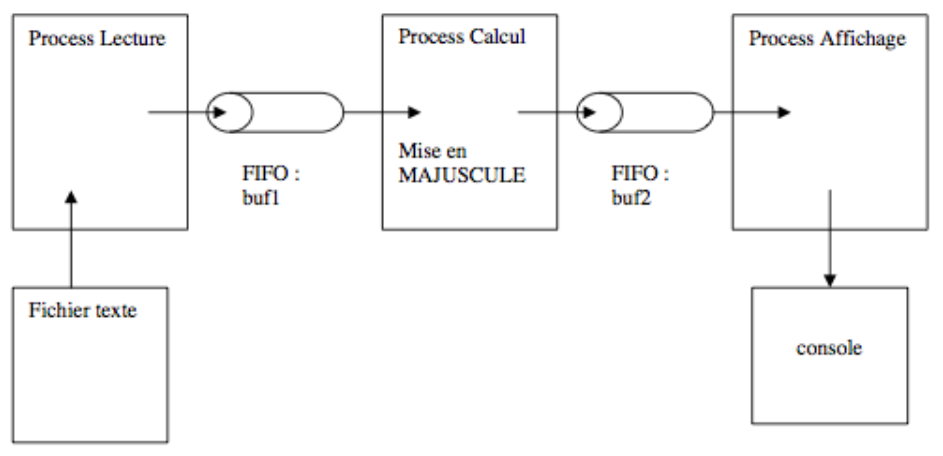
\includegraphics[width=.8\textwidth]{./screenshots/enonce.png}
        \end{figure}
        \begin{itemize}[label=\textbullet]
            \item Le thread \emph{Lecture} sera implémenté par une fonction et lira un fichier texte caractère par caractère. Chaque caractère lu sera ajouté à la FIFO \emph{buf1}.
            \item Le thread \emph{Calcul} sera implémenté par une fonction et lira ses données hors de la FIFO \emph{buf1}. Chaque caractère lu sera alors converti en majuscule avant d'être envoyé dans la FIFO \emph{buf2}.
            \item Le thread \emph{Affichage} sera implémenté par une fonction et lira ses données hors de la FIFO \emph{buf2}. Chaque caractère lu sera affiché sur la console.
        \end{itemize}
        \item Gérer les protections en cas de sur et sous alimentation des FIFO à l'aide de sémaphores au sein du code de la FIFO.
        \item Tester votre programme avec différentes tailles de FIFO (N=1, N=2, N=10, ...)
        \item Dessiner un diagramme temporel montrant le séquencement de cotre programme.
    \end{enumerate}

    \newpage
    \section{Diagramme de séquence}

    \begin{figure}[H]
        \centering
        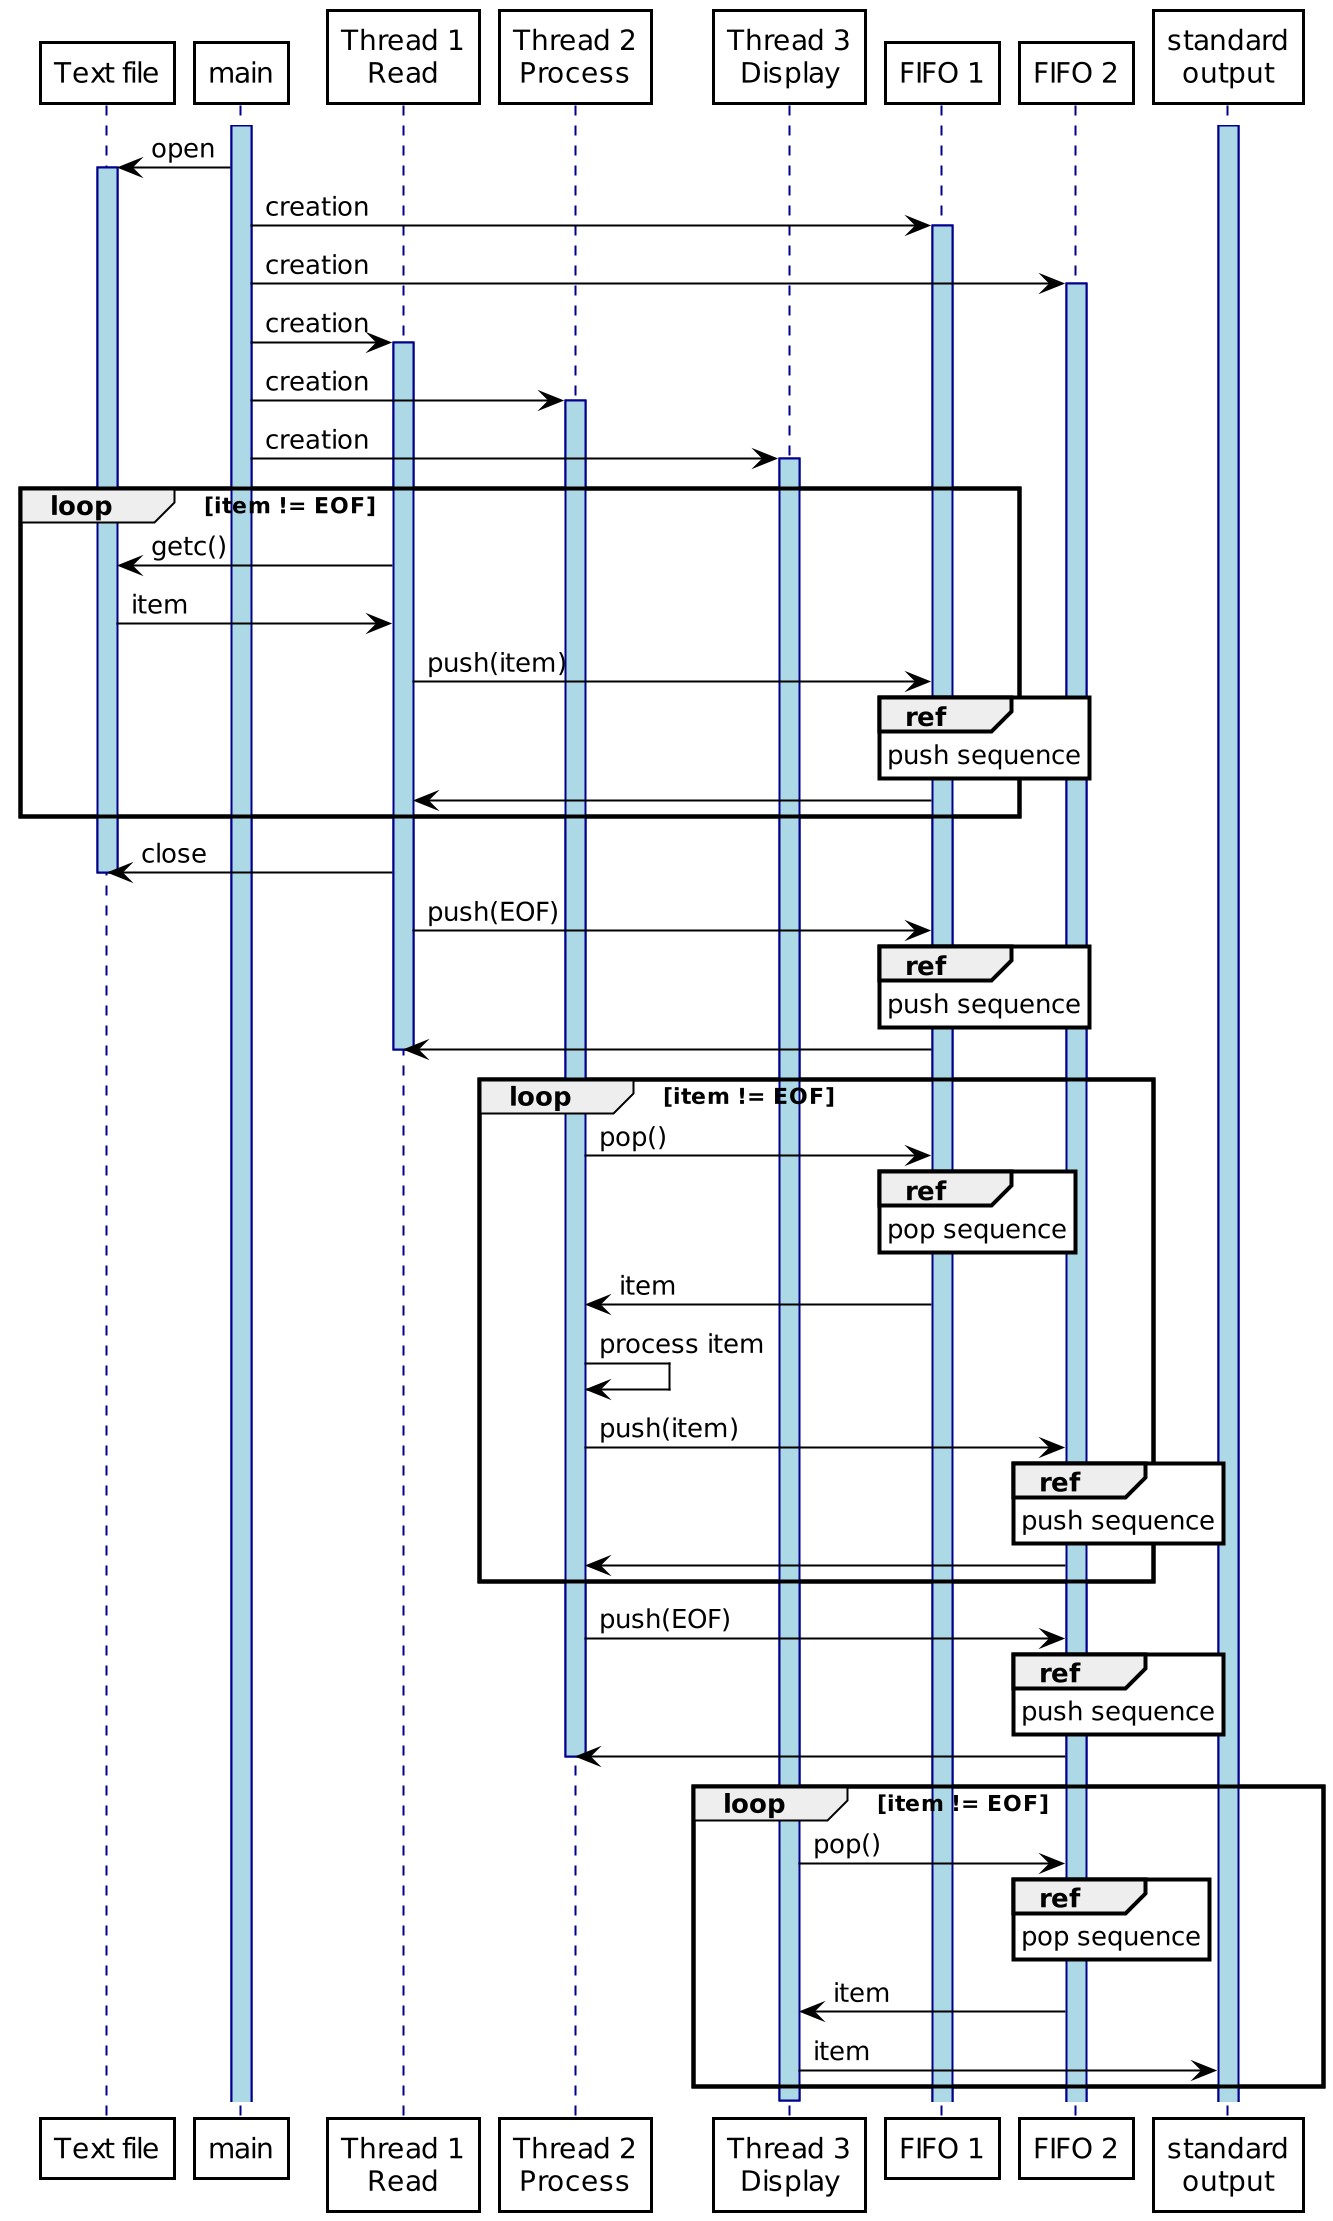
\includegraphics[width=.65\textwidth]{./diagrammes/sequence_full/prodcon-full-sequence.png}
    \end{figure}

    \paragraph{}
    Les trois threads sont activés en même temps (lors de leur création par le \texttt{main}). Cela signifie par exemple que le thread \emph{Process} peut appeler la fonction \texttt{pop()} de manière concurrente au \texttt{push()} du thread \emph{Read}. C'est au sein de ces méthodes que sont implémentées l'attente d'un item disponible avant de le récupérer ou l'attente d'un espace libre avant d'insérer un nouvel item dans le buffer.

    \paragraph{}
    Un même thread ne peut par contre pas lancer plusieurs \texttt{push(item)} ou \texttt{pop()} en parallèle : ces méthodes bloquent le thread et doivent se terminer avant que le thread ne puisse continuer.

    \paragraph{}
    Le thread \emph{Read} lit les caractères du fichier texte donné en paramètre au programme et les ajoute un à un à la \emph{FIFO 1}. Le caractère \texttt{EOF} est lui aussi envoyé à la FIFO pour que le second thread sache quand s'arrêter. Il s'arrête alors.
    
    \paragraph{}
    Le thread \emph{Process} lit un à un les caractères de la \emph{FIFO 1} pour les mettre en majuscules et les insérer dans la \emph{FIFO 2}. Ce thread envoie lui aussi le caractère \texttt{EOF} à la \emph{FIFO 2} avant de s'arrêter.

    \paragraph{}
    Le thread \emph{Display} lit les caractères de la \emph{FIFO 2} un à un et les affiche en console. Il s'arrête dès qu'il a lu le caractère \texttt{EOF}.

    \begin{figure}[H]
        \centering
        \begin{subfigure}[b]{.48\textwidth}
            \centering
            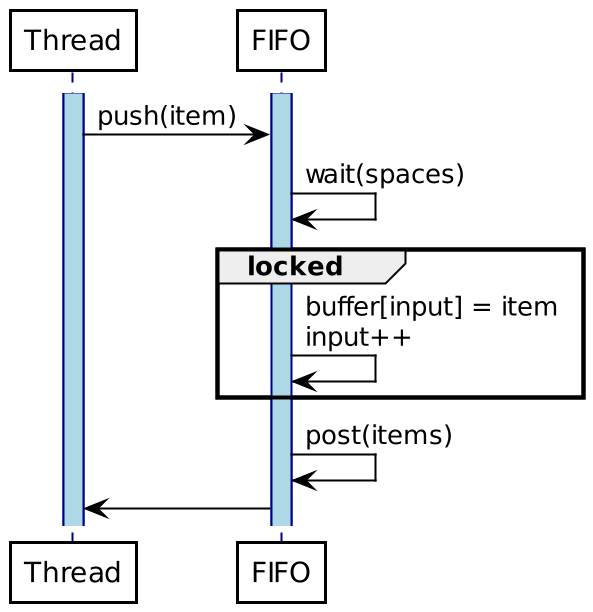
\includegraphics[width=.74\textwidth]{./diagrammes/sequence_push/prodcon-push-sequence.png}
            \caption{push sequence}
        \end{subfigure}
        \begin{subfigure}[b]{.48\textwidth}
            \centering
            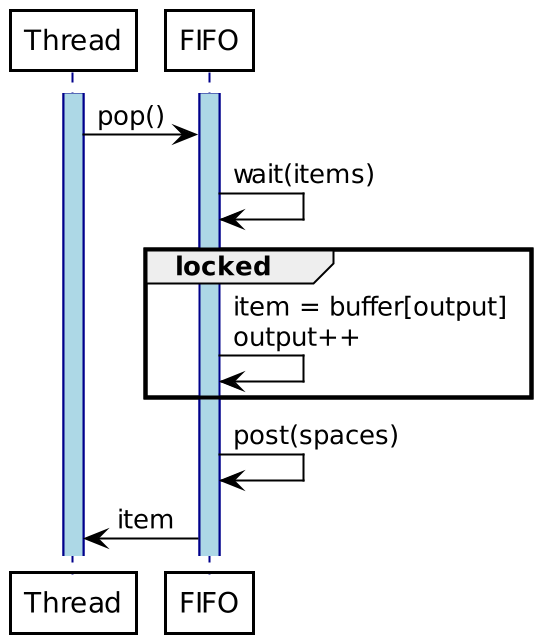
\includegraphics[width=.65\textwidth]{./diagrammes/sequence_pop/prodcon-pop-sequence.png}
            \caption{pop sequence}
        \end{subfigure}
    \end{figure}


    \paragraph{}
    Les FIFO gèrent la protection de l'accès à leurs buffers par un mutex. Pour éviter de bloquer la lecture du buffer alors qu'il est vide, le sémaphore \texttt{items}, initialisé à 0, est incrémenté à chaque fois qu'un nouvel item est inséré dans le buffer et décrémenté à chaque fois qu'un item est lu. Pour éviter l'insertion d'un item dans un buffer déjà plein, le sémaphore \texttt{spaces}, initialisé à la taille du buffer, est décrémenté à chaque fois qu'un item est ajouté au buffer et incrémenté à chaque fois qu'un item est lu.

    \newpage
    \section{Compilation}
    La compilation est réalisée en utilisant cmake via le fichier \emph{CMakeLists.txt} :
    \begin{verbatimtab}
    [1]     cmake_minimum_required(VERSION 3.10)

    [2]     project(Exercice2_Producteurs_Consommateurs VERSION 1.0)

    [3]     set(CMAKE_C_FLAGS "${CMAKE_C_FLAGS} -Wall -Wpedantic -Wextra")

    [4]     include_directories(PUBLIC include)

    [5]     set(SOURCE_FILES
                src/prodcon.c
                src/fifo.c)

    [6]     find_package(Threads REQUIRED)

    [7]     add_executable(prodcon ${SOURCE_FILES})

    [8]     target_link_libraries(prodcon PRIVATE Threads::Threads)
    \end{verbatimtab}

    \begin{description}
        \item[\texttt{[1]}] version de \texttt{cmake} utilisée
        \item[\texttt{[2]}] nom et version du projet
        \item[\texttt{[3]}] ajout des flags habituels pour l'affichage de tous les warnings
        \item[\texttt{[4]}] le répertoire \emph{include} contient les headers nécessaires à la compilation
        \item[\texttt{[5]}] définition de la variable \texttt{SOURCE\_FILES} contenant les fichiers sources du projet
        \item[\texttt{[6]}] ajout du package pour l'utilisation des threads
        \item[\texttt{[7]}] la compilation des fichiers sources produit l'exécutable \texttt{prodcon} 
        \item[\texttt{[8]}] le projet utilise la librairie \texttt{Threads} du package \texttt{Threads}
    \end{description}

    \newpage
    \paragraph{}
    La commande \texttt{cmake ..} lancée depuis le sous-répertoire \emph{build} permet de générer le \emph{Makefile} :
    \begin{figure}[H]
        \centering
        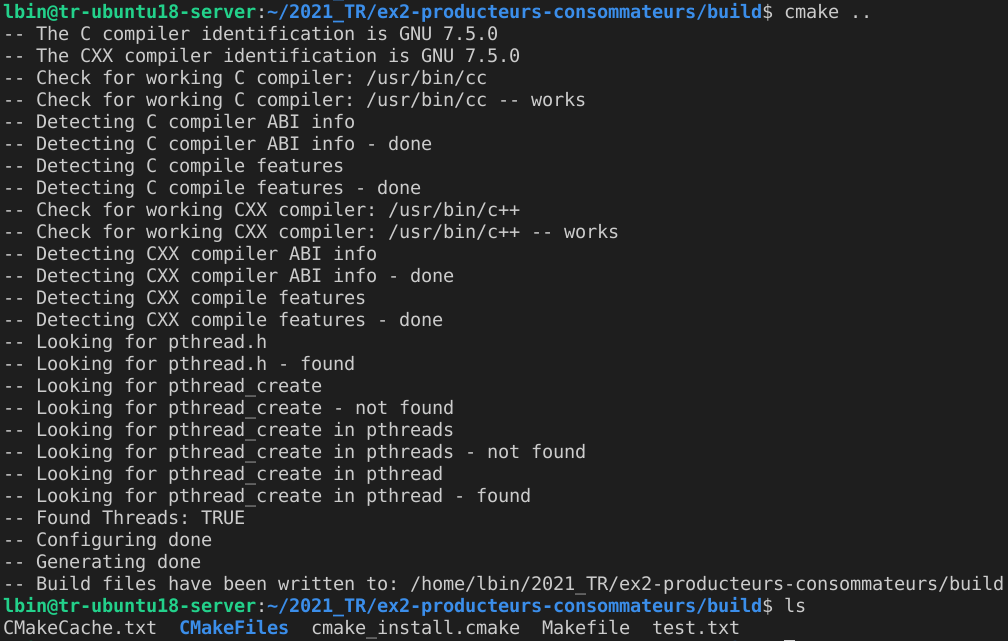
\includegraphics[width=.8\textwidth]{./screenshots/cmake.png}
    \end{figure}

    \paragraph{}
    Par défaut, le \emph{Makefile} est généré en mode debug. Pour le générer en mode release, j'utilise la commande \texttt{cmake -DCMAKE\_BUILD\_TYPE=Release \emph{path}}, où \texttt{\emph{path}} est l'endroit où se trouve le fichier \emph{CMakeLists.txt}.
    
    \paragraph{}
    La commande \texttt{make} me permet de compiler le projet à partir du \emph{Makefile} pour produire l'exécutable \emph{prodcon} :
    \begin{figure}[H]
        \centering
        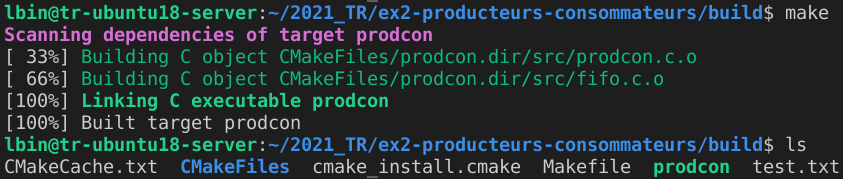
\includegraphics[width=.65\textwidth]{./screenshots/make.png}
    \end{figure}

    \newpage
    \section{Tests}
    \paragraph{}
    Le programme est testé avec des temporisations aléatoires dans les threads (entre 1 et \SI{20000}{\micro\second}). Il attend en paramètres le nom du fichier à lire et la taille des buffers :
    \begin{figure}[H]
        \centering
        \begin{subfigure}[b]{.48\textwidth}
            \centering
            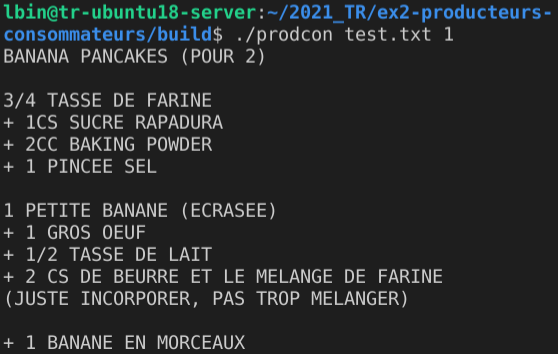
\includegraphics[width=\textwidth]{./screenshots/test1.png}
        \end{subfigure}
        \begin{subfigure}[b]{.48\textwidth}
            \centering
            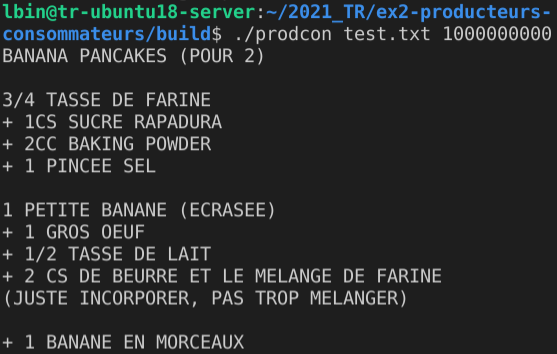
\includegraphics[width=\textwidth]{./screenshots/test1000000000.png}
        \end{subfigure}
    \end{figure}

    \paragraph{}
    Fichier d'origine utilisé pour le test :
    \begin{figure}[H]
        \centering
        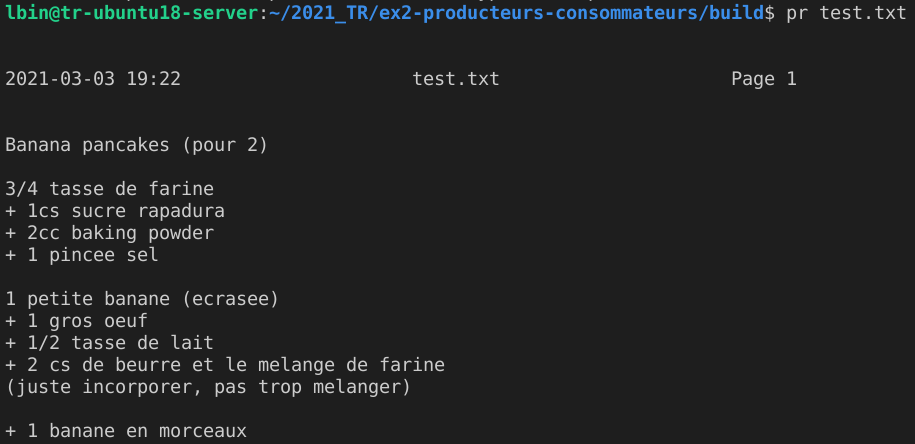
\includegraphics[width=.8\textwidth]{./screenshots/test_text.png}
    \end{figure}
\end{document}
